\section{Time series clustering}

Aside from motion tracking, time series data is prevalent in numerous data mining applications, from weather forecasting to energy consumption predictions. In many scenarios, clustering techniques serve as a wonderful exploratory tool to group either similar time series altogether, or to obtain segments in single instances in which the data behaves in consistently similar ways \cite{ChristopherMBishop2006PatternLearning}.

In the general case, we consider a set of N objects represented as:

\begin{equation}
X = \{x_1, \ldots, x_N\}
\label{eq:2.1}
\end{equation}

Taking a measure of dissimilarity between objects $x_i$ and $x_j$ that can be expressed as $d(x_i, x_j)$, the goal of clustering is to divide $X$ into a partition $C = {c_1, ..., c_k}$ consisting of $K$ clusters, which maximizes both the similarity between objects within the same cluster, and the dissimilarity between objects in different clusters \cite{Lafabregue2022End-to-endStudy}. 

The overall objective of clustering in the context of this thesis, therefore, is to find a mapping function $f_\Theta$ that enables the obtaining of a relevant partition $C$ for time series data. Unlike many other data types, however, time series have some peculiarities that make this problem exceptionally hard, and render traditional algorithms unsuitable without either pertinent modification or data preprocessing. To explore why this is the case, let us represent a time series of length $T$ as:

\begin{equation}
x_i = [x_{i,1}, x_{i,2}, \ldots, x_{i,T}]
\label{eq:2.2}
\end{equation}

Here, $x_i \in \mathbb{R}^{(d \times T)}$, where $d$ is the number of features for each time step. Series with $d = 1$ are considered univariate, and series with $d > 1$ (as virtually all cases explored in this thesis) are deemed multivariate. That said, the unique nature of the time dimension presents challenges when employing traditional clustering methods. For starters, each time step cannot be regarded as an independent feature, with observations displaying varying degrees of autocorrelation \cite{Murphy2022ProbabilisticIntroduction}. Furthermore, two time series may represent similar objects, but their time signals could be delayed, stretched, or affected by noise (Figure~\ref{fig:2.1}). Consequently, these time series may exhibit significant differences in Euclidean space, despite representing similar signals \cite{Lafabregue2022End-to-endStudy}. As a result, researchers have proposed a plethora of time series-specific clustering methods in the literature.

Along these lines, more classical methods tend to rely on adapting time series to the Euclidean space through time-aware feature extraction \cite{Christ2018TimePackage}, or to design alternative distance metrics that can take care of alignment issues \cite{Tavenard2021AnWarping}. While these methods are widely used for their simplicity and interpretability, they may struggle with high dimensional or noisy data (such as motion tracking), and can be computationally expensive for large datasets.

As an intermediate methods' family, probabilistic models, such as Hidden Markov Models (HMMs) retain some interpretability capabilities, while excelling at time segmentation even for time series with several dimensions. They typically exhibit difficulties handling long-range dependencies, however, due to the underlying Markovian assumption \cite{Murphy2022ProbabilisticIntroduction}, and are in general less robust to noise than other alternatives, requiring specific tweaks tailored to each specific situation \cite{Weinreb2023Keypoint-MoSeq:Dynamics}.

On the other hand, neural network-based methods have gained popularity for their ability to automatically learn complex features from the data \cite{Lafabregue2022End-to-endStudy}. These methods excel at handling high dimensional and noisy time series, and are capable of capturing long-range dependencies. However, they can be more challenging to interpret, require larger datasets for training, and may be prone to overfitting if not properly regularized.

In the following sections, we discuss in detail the primary time series clustering methods available in the literature, as well as their advantages and disadvantages in general and for motion tracking data in particular. A set of specific behavioral segmentation examples across many of these categories are provided, and the main ideas to explore in the algorithms presented in this thesis are introduced.

\begin{figure}[!thb]
\centering
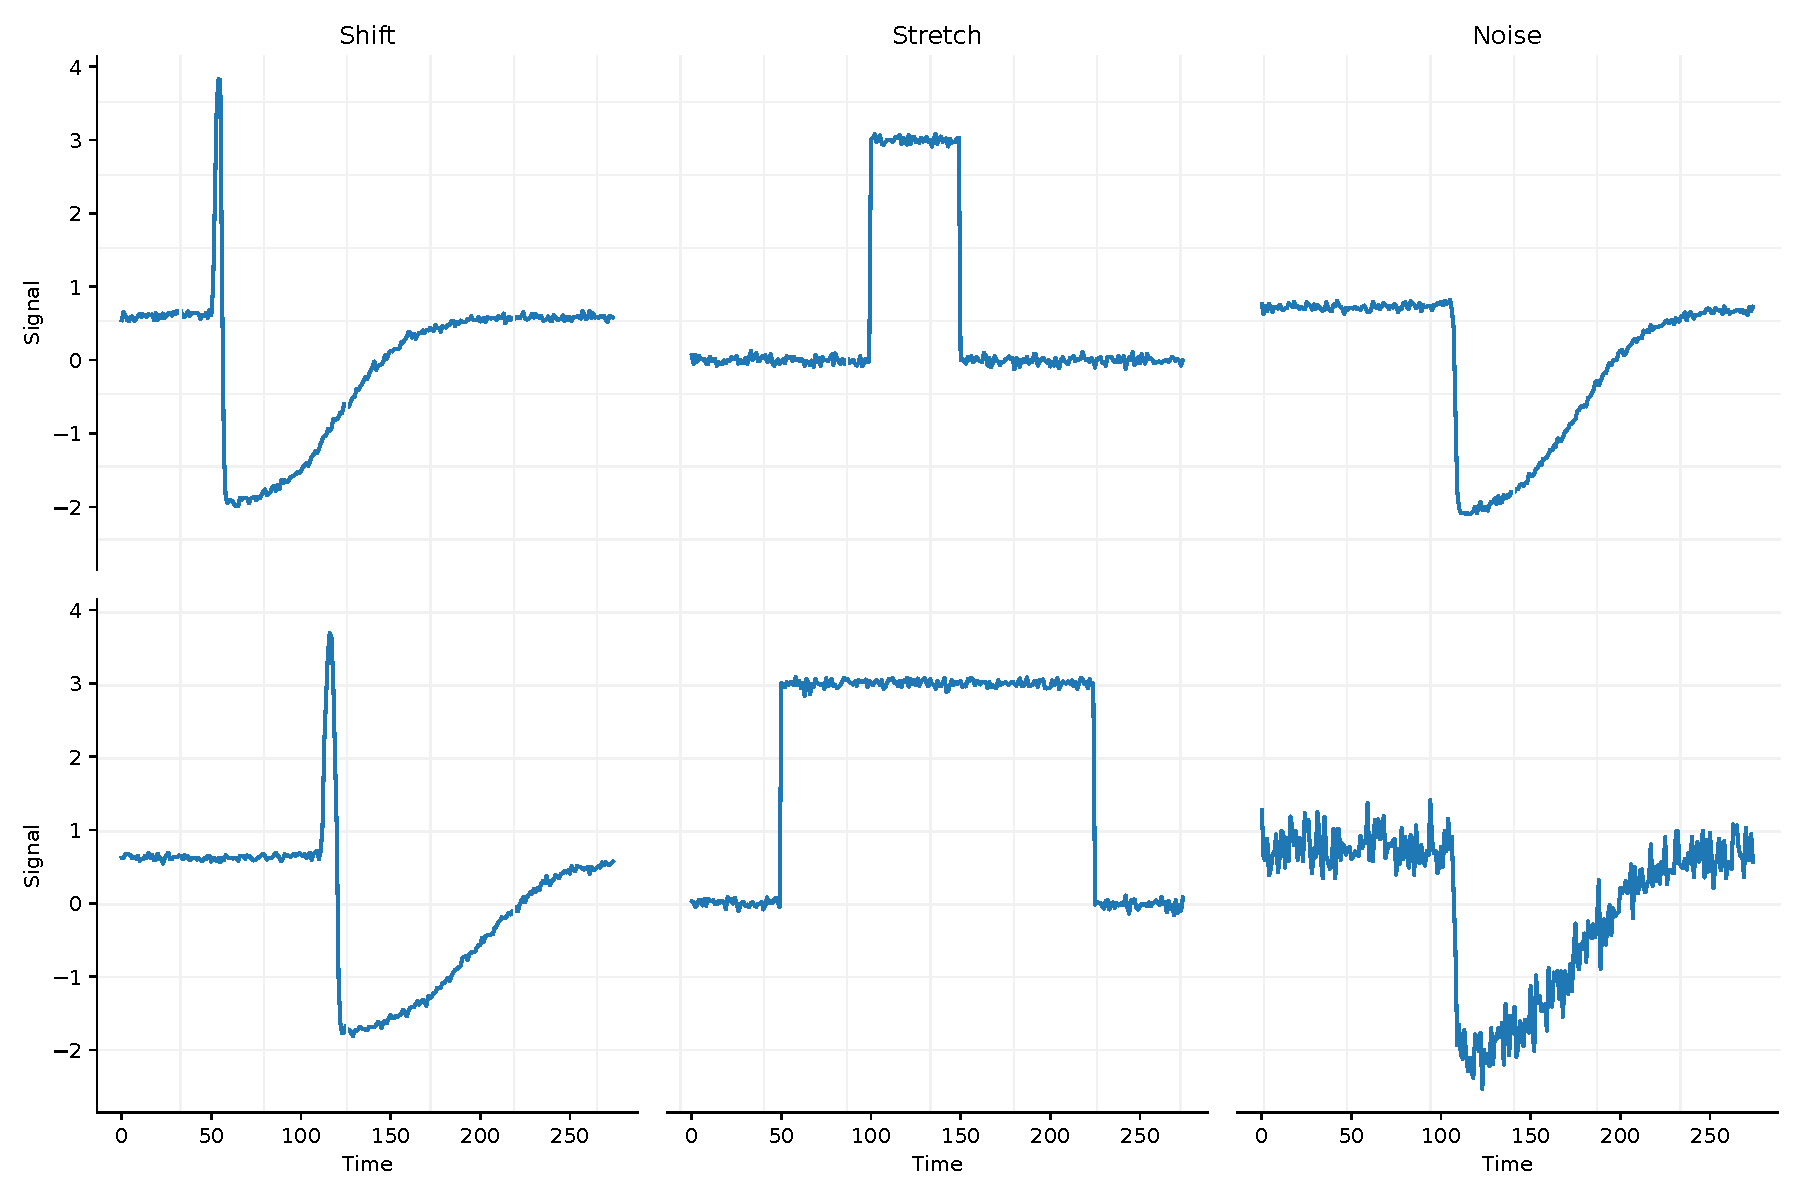
\includegraphics[width=\textwidth]{Figures/sota_1.pdf}

\caption[\textbf{Issues with time series clustering in Euclidean space}]{\textbf{Issues with time series clustering in Euclidean space:} Examples of time series belonging to the same class with time shifts (left-most column) stretches
(central column) or varying noise (right-most column). (Adapted from \cite{Lafabregue2022End-to-endStudy}).}
\label{fig:2.1}

\end{figure}

\subsection{Classical methods}

As previously mentioned, unsupervised learning methods in machine learning provide a way to explore and understand the intrinsic structure of data without labeled information or predetermined categories. For time series in particular, special care must be taken to deal with issues such as autocorrelation in the time dimension. In this section, we explore classical approaches (that is, algorithms that do not rely on neural networks) to take care of this issue in time series segmentation, including time-aware feature extraction, specific distance metrics (such as DTW) and HMMs.

\subsubsection{Classical clustering using time-aware feature extraction}

The first approach to explore aims to collapse the time dimension using feature extraction techniques, thus reducing two-dimensional matrices (where dimensions correspond to time and features) to vectors that can be fed to classical dimensionality reduction and clustering algorithms.

This is accomplished by extracting meaningful and representative features that capture the essential patterns and characteristics of the data. Some commonly used feature extraction methods include statistical measures (such as mean, variance, skewness, and kurtosis), frequency domain features (such as Fourier and wavelet transforms), and time-domain features (such as autocorrelation, trend, and seasonality) \cite{Fulcher2017Feature-basedAnalysis}. 

Once features are extracted, classical clustering algorithms, such as K-means, hierarchical clustering, or density-based spatial clustering of applications with noise (DBSCAN), can be applied to group similar time series based on their extracted features \cite{ChristopherMBishop2006PatternLearning}. As customary with non-time-series data as well, and given the vast number of extracted features in some cases \cite{Christ2018TimePackage} high-dimensional vectors are usually reduced to lower-dimensional manifolds using dimensionality reduction techniques such as Principal Component Analysis (PCA), or Uniform Manifold Approximation and Projection (UMAP) \cite{Xia2021RevisitingStudy, McInnes2018UMAP:Reduction}. This helps deal with the so-called ``curse of dimensionality", a phenomenon describing how common distance metrics are not suitable for grouping patterns in high-dimensional spaces \cite{Murphy2022ProbabilisticIntroduction}.

Thus and so, this approach enables the use of well-established clustering techniques on time series data while reducing computational complexity and mitigating challenges associated with the time-dependent nature of the data. However, the success of these kinds of pipelines largely depends on the choice of features and their ability to represent the intrinsic structure of the time series data effectively \cite{Enes2023AJobs, Petelin2023TowardsPrediction}. Moreover, for large datasets feature extraction itself can become cumbersome in terms of computational complexity, deeming other methods usually more suitable \cite{Petelin2023TowardsPrediction}.

The standard pipeline included in the python package tsfresh (Time Series FeatuRe Extraction on basis of Scalable Hypothesis tests) is a good example of this kind of approaches in practice. It applies 63 time series characterization methods, which (using default parameters) output a series of 794 features per dimension. Furthermore, it offers domain specific subsets of features, and task-specific feature selection pipelines such as statistical testing for supervised learning, and variance-based methods for clustering \cite{Christ2018TimePackage} (Figure~\ref{fig:2.2}).

\begin{figure}[!thb]
\centering
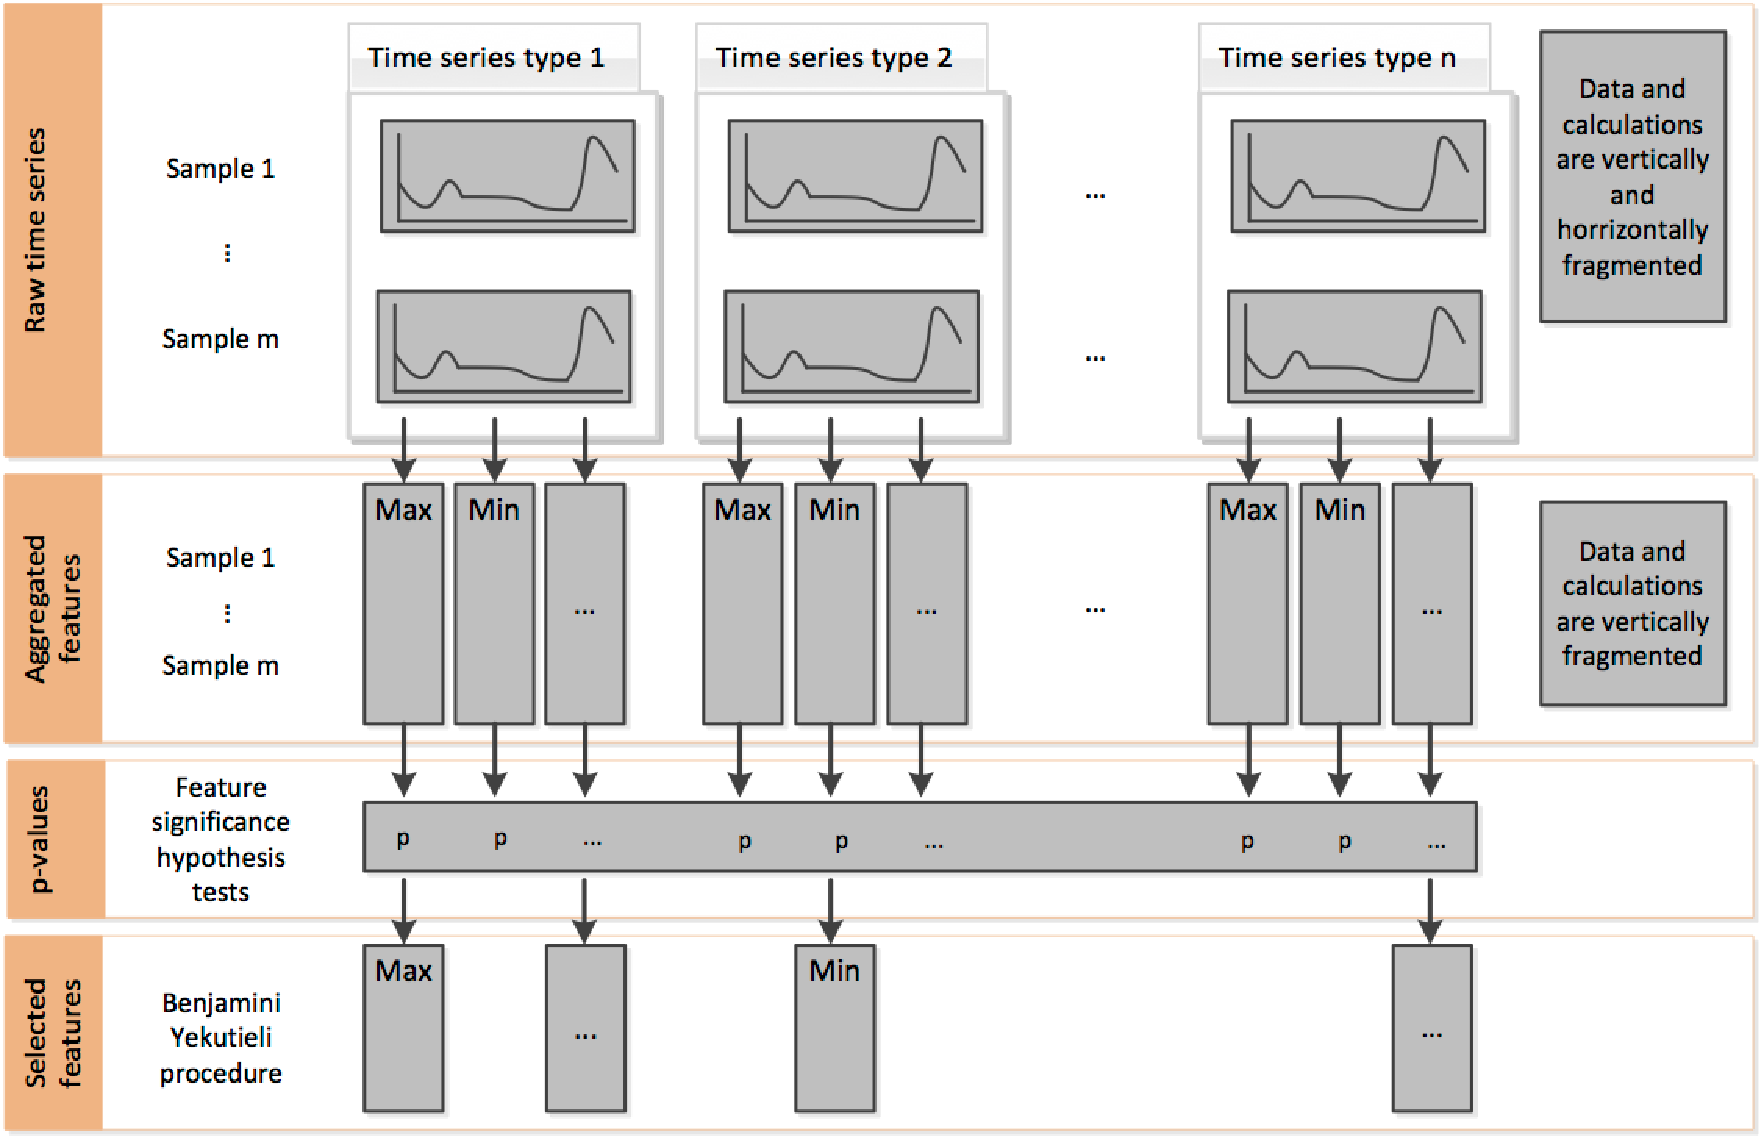
\includegraphics[width=\textwidth]{Figures/sota_2.pdf}

\caption[\textbf{An overview of the tsfresh feature extraction pipeline}]{\textbf{An overview of the tsfresh feature extraction pipeline:} Starting with the analysis of time series, the algorithm uses established feature mappings and includes extra meta-information features. When focused on supervised learning tasks, each feature is individually assessed to gauge its predictive importance for the target in question. The process involves statistical testing and $p$-value adjusting for multiple comparisons, which helps decide which features should be retained. In contrast, for unsupervised learning tasks, the algorithm applies variance-based filters on the features. (Adapted from \cite{Christ2018TimePackage}).}
\label{fig:2.2}

\end{figure}

\subsubsection{Dynamic Time Warping and temporal K-Means}

While the approach described so far aimed to adapt time series to work with already established clustering methods, this section deals with the arguably opposite approach: by defining suitable distance metrics, algorithms can be adapted to work with time series data without the need for custom feature extraction pipelines. This eliminates the need for domain knowledge or extensive experimentation to identify the most representative features, which can be a time-consuming process.

Along these lines, Dynamic Time Warping (DTW) is a powerful technique for measuring the similarity between two time series, allowing for non-linear alignments that can account for variations in the timing and speed of patterns within the data. DTW works by dynamically aligning the sequences and calculating the optimal distance between them, taking into account potential time shifts and warping of the series (Figure~\ref{fig:2.3}).

Formally, let us consider two time series $x$ and $x'$, where all elements $x_i$ and $x'_j$ lie in the same $d$-dimensional space. The exact points in time where patterns occur are ignored, and just the ordering of the sequence matters.

The algorithm then searches for the alignment that minimizes the Euclidean distance between two time series:

\begin{equation}
\mathrm{DTW}_q({x}, {x}^\prime) =
    \min_{\pi \in \mathcal{A}({x}, {x}^\prime)}
        \left( \sum_{(i, j) \in \pi} d(x_i, x^\prime_j)^q \right)^{\frac{1}{q}}
\label{eq:2.3}
\end{equation}

where $\pi$ is an alignment path of length $K$ (a sequence of $K$ index pairs), and $A(x, x')$ is the set of all admissible paths (where indices are monotonically increasing, and start and end of both time series match) \cite{Tavenard2021AnWarping, Vintsyuk1968SpeechProgramming, Itakura1975MinimumRecognition, Sakoe1978DynamicRecognition}. All in all, the algorithm returns distances that are always positive (DTW$_q({x}, {x}^\prime) \geq 0$) for any time series $x$ and $x'$. Moreover, the DTW distance between any time series and itself is always zero (DTW$_q({x}, {x}) = 0$).

When applied to clustering, the most commonly used algorithm is known as temporal K-means, which is an adaptation of the K-means algorithm that (among other modifications, such as DTW Barycenter Averaging) uses DTW as a distance metric instead of its Euclidean counterpart \cite{Petitjean2011AClustering}. Interestingly, when compared to the previously described approaches, DTW-based methods tend to be less sensitive to noise in the data. However, they are also less prone to detecting changes in amplitude, as they focus on the overall shape of the time series. Furthermore, DTW-based methods can be computationally expensive, particularly for large datasets or long time series, as they require calculating pairwise distances between all data points in the sequences (although this can be mitigated by applying bounding techniques to prune the search space \cite{Tralie2020ExactMemory}). All in all, DTW remains a popular choice for time series clustering due to its flexibility and ability to capture complex relationships within the data.

Finally, it is worth mentioning that the approaches described so far aim in principle to group time series rather than to find segments within them. This can be solved, however, by extracting sliding windows within a given time series, as will be explored in more detail later in this and the following chapter \cite{Hsu2021B-SOiDBehaviors, Luxem2022IdentifyingMotion}. The next section deals with Hidden Markov Models (HMMs), a set of approaches which can, among other things, handle segmentation tasks directly, without the need for sliding window extraction.

\begin{figure}[!thb]
\centering
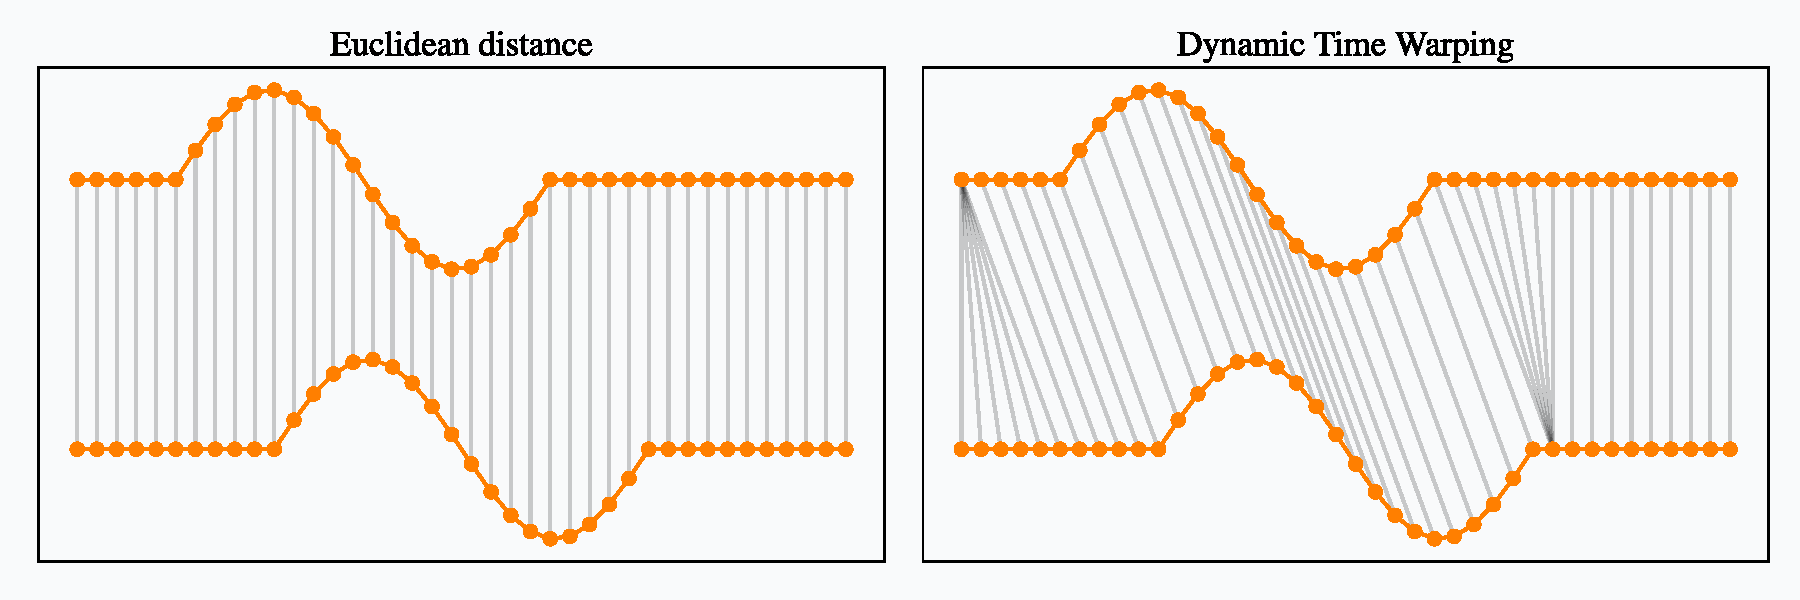
\includegraphics[width=\textwidth]{Figures/sota_3.pdf}

\caption[\textbf{Comparison between DTW and Euclidean distance}]{\textbf{Comparison between DTW and Euclidean distance:} Comparison between two time series using either Euclidean distance (shown on the left) or Dynamic Time Warping (DTW, shown on the right), the latter being a classic example of an alignment-based metric. In both scenarios, the computed similarity is the cumulative distance between corresponding features (indicated by the gray lines). It is noteworthy how DTW aligns distinctive patterns in the time series, which results in a method that is likely to provide a more reliable evaluation of similarity for time series than the Euclidean distance approach, which aligns timestamps irrespective of their feature values. (Adapted from \cite{Tavenard2021AnWarping}).}
\label{fig:2.3}

\end{figure}

\subsubsection{Hidden Markov Models}

Hidden Markov Models fall in the category of probabilistic graphical models (PGMs), which model sets of (observed or latent) variables as a joint probability distribution in a way that aims to encode conditional independence assumptions using a graph structure \cite{Murphy2022ProbabilisticIntroduction}. 

The fundamental concept in PGMs is that every node in the graph symbolizes a random variable, and each edge signifies a direct dependency. Furthermore, the absence of an edge indicates conditional independence between two variables. In the case of a directed acyclic graph (DAG, often referred to as a Bayesian network), the nodes can be arranged in topological order (with parents preceding their children) and connected in such a way that each node is conditionally independent of its predecessors, given its parent nodes:

\begin{equation}
Y_i \perp Y_{\mathrm{pred}_i \setminus \mathrm{pa_i}} \mid Y_{\mathrm{pa}_i}
\label{eq:2.4}
\end{equation}

\noindent where $pa_i$ are the parents of node $i$, and $pred_i$ are the predecessors of node $i$ in the given ordering. The joint distribution can thus be represented as follows:

\begin{equation}
p(Y_1:N_G) = \prod_{i=1}^{N_G} p(Y_i | Y_{\mathrm{pa}_i})
\label{eq:2.5}
\end{equation}

\noindent where $N_G$ is the number of nodes in the graph.

Along these lines, an HMM is a graphical model that models observations across time ($y$) as coming from a set of latent discrete states ($z$). Once trained, the model will assign a state to each time point in the series, which depends both on the observations available for that time point, and on the state assigned to the time point that came just before (Figure~\ref{fig:2.4}, \textbf{a}). This last statement corresponds to the Markov assumption, which applies to the latent (hidden) variables, hence the name of the models. Formally, the joint probability of the model can be represented as:

\begin{equation}
p(y_1:T, z_1:T) = p(z_1) \prod_{t=2}^{T} p(z_t|z_{t-1}) \prod_{t=1}^{T} p(y_t|z_t)
\label{eq:2.6}
\end{equation}

\noindent where $z_t$ are the hidden variables, and $y_t$ are the observations (outputs) at time $t$. In practice, training such models requires learning probability distributions describing each of the states (called emission distributions), as well as a transition matrix describing the probability of any given state transition. As an example, a hidden Markov model with two states could be applied to represent the rolls of a fair and a loaded dice (respectively) in a casino. By estimating the transition probabilities between the states, a model like this could enable the identification of possible cheating or unfair play given a sequence of dice rolls \cite{Murphy2022ProbabilisticIntroduction} (Figure \ref{fig:2.4}, \textbf{b}).

\begin{figure}[!thb]
\centering
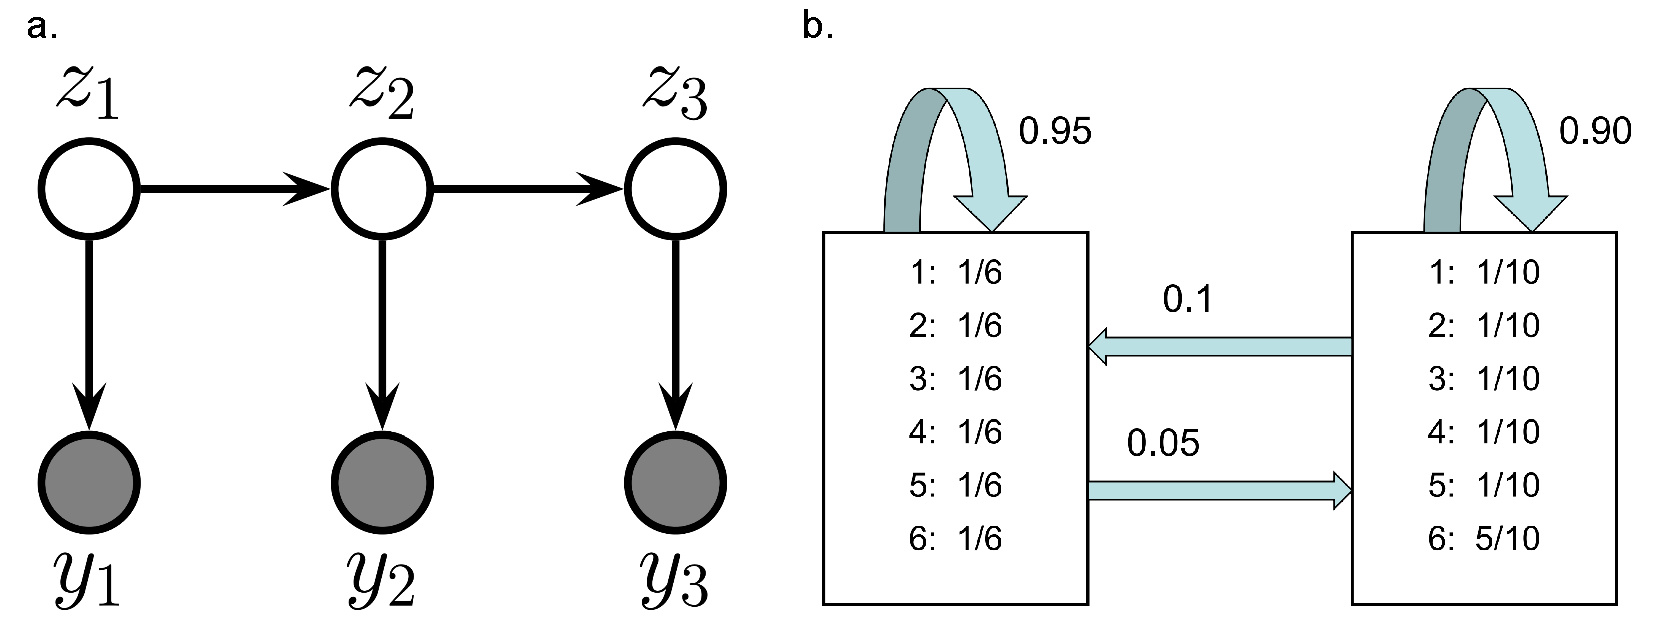
\includegraphics[width=\textwidth]{Figures/sota_4.pdf}

\caption[\textbf{Hidden Markov Models (HMMs)}]{\textbf{Hidden Markov Models (HMMs):} \textbf{a.} An HMM represented as a graphical model, where $z_t$ are the hidden variables at time $t$, and $y_t$ are the observations (outputs). \textbf{b.} State probabilities for a fair and a loaded dice (left and right, respectively), alongside transition probabilities between them (light blue arrows). (Adapted from \cite{Murphy2023ProbabilisticTopics}).}
\label{fig:2.4}

\end{figure}

As previously introduced, an advantage of these models when compared to the previously discussed approaches is that HMMs segment each time series directly, without the need to discretize the time dimension using sliding windows. Moreover, the parametric nature of the models has strong advantages when it comes to interpretability, as each state is described by probability distributions that can be mapped back to the data. However, these advantages come at the expense of flexibility, as long range dependencies in the data are lost by definition. While extensions to these models have been developed to mitigate this issue, their correct implementation requires domain expertise and may not be applicable to all scenarios \cite{Weinreb2023Keypoint-MoSeq:Dynamics, Mor2021AApplications}.

In strong contrast to this idea, the next section delves into the use of neural networks to model time dependencies, and into the existing deep learning algorithms for time series clustering and segmentation. Interestingly, these models follow the opposite trend as HMMs: while neural networks are universal function approximators that arguably champion flexibility, their interpretation often requires significantly more effort \cite{Roberts2021TheTheory}.

\subsection{Deep clustering}

Representation learning is a subfield of machine learning that focuses on finding transformations that can automatically discover abstract, meaningful features from raw data \cite{Roberts2021TheTheory}. These features can then be used to improve the performance of various tasks such as classification, regression, and clustering. Moreover, deep neural networks (DNNs) are capable of capturing complex patterns and hierarchical structures in the data, making them extremely useful for learning meaningful representations.

Thus and so, and in contrast to the methods presented so far, deep learning approaches for clustering typically involve learning a representation of the data and performing clustering on the result of this transformation rather than on the raw data, either jointly or in a post-hoc fashion \cite{Lafabregue2022End-to-endStudy}. This representation is obtained by encoding the data with a DNN (referred to as an encoder) capable of acting as a non-linear mapping function $f_\Theta :X\rightarrow Z$, where $\Theta$ represents all learnable parameters. These models can thus learn  $Z$ as a representation of $X$, which is called the latent (or hidden) space. The clustering task then involves partitioning the set $Z$, such that:

\begin{equation}
Z = \{z_1, \ldots, z_N\} = \{f_\Theta(x_1), \ldots, f_\Theta(x_N)\}
\label{eq:2.7}
\end{equation}

\noindent where the partition is defined over $Z$ (which in turn is a function of $X$) instead of over $X$ directly as presented in equation \ref{eq:2.1}. Moreover, network architectures, the data and its processing, as well as training schemes used are crucial to a successful representation.

Along these lines, an extremely popular architecture for representation learning has been the deep autoencoder. Its basic architecture consists of two parts: an encoder that maps the input data to a lower-dimensional latent space $f_{\Theta} : X \rightarrow Z$, and a decoder that reconstructs the input data from the latent representation $g_{\Theta} : Z \rightarrow y$~\cite{Rubio2023Auto-EncodersPerspectives}. The objective of an autoencoder is then to minimize the reconstruction error of the input given the output $p(X|y)$ while forcing the data through a series of bottleneck layers that impose constraints in the model, preventing it from learning trivial solutions such as the identity function. Moreover, adaptations such as the Variational Autoencoder \cite{Kingma2013Auto-EncodingBayes} enabled its effective use for representation learning and data generation, since the latent space can be interpreted as a probability distribution.

Another popular approach for representation learning is contrastive learning, which works using an encoder only, by optimizing a contrastive loss function that encourages the model to pull together positive pairs (similar instances) and push apart negative pairs (dissimilar instances). This set of approaches has been particularly successful in self-supervised learning scenarios, where large amounts of unlabeled data are leveraged to learn useful representations \cite{Le-Khac2020ContrastiveReview}.

Furthermore, and while representation learning is a crucial step of the pipeline, deep clustering goes a step further by aiming to segment the learned manifolds into meaningful subgroups. Either by learning representations that facilitate clustering and segmenting afterward or by training a clustering solution jointly with the representation, these approaches have several advantages. Besides the ability to learn non-linear transformations of the data, which can lead to better cluster separation, they can automatically discover hierarchical structures in the data, and be more robust to noise and irrelevant features due to the hierarchical nature of the learned representations. Moreover, end-to-end models allow for back-propagation of the clustering structure through the encoder, priming the network as a whole to yield representations that have a cluster structure \cite{Lafabregue2022End-to-endStudy}.

Before delving into deep clustering itself in the following chapters, the next sections aim to establish a common ground on the building blocks of working with time series and deep neural networks. Three architectural paradigms are presented, including Recurrent Neural Networks (RNNs), Temporal Convolutional Networks (TCNs), and Transformer networks.

\subsubsection{Recurrent Neural Networks}

Recurrent Neural Networks (RNNs) are a class of deep learning models specifically designed to handle sequential data, which makes them highly applicable for tasks involving time series analysis \cite{Lipton2015ALearning}. The core feature of an RNN is its ability to maintain a hidden state that captures information from previous time steps, allowing any given model to effectively process and learn from temporal dependencies within the data. This structure enables RNNs to excel in a wide range of applications, such as natural language processing, speech recognition, and, as this section suggests, time series representation in general.

They have the particularity that the sequence is fed step by step to the layer, updating a common hidden state, which serves as a memory of preceding steps. Thus, the layer consists of a recursive function $g$ that takes the current data step $x_t$ and the previous hidden state $h_t$ to generate the new updated hidden state:

\begin{equation}
h_t = g(x_t, h_{t-1})
\label{eq:2.8}
\end{equation}

\noindent where $h_0$ is typically initialized with zeros. The original recursive function was defined as:

\begin{equation}
h_t = \tanh(W x_t + U h_{t-1} + b)
\label{eq:2.9}
\end{equation}

\noindent where $h_t$ is a vector of size $u$, with $W \in \mathbb{R}^{u \times d}$ and $U \in \mathbb{R}^{u \times u}$ representing the weights, and $b \in \mathbb{R}^u$ denoting the bias vector learned during training. While useful in many cases, this cell type often results in vanishing gradients, making training difficult and long-range dependency learning hard \cite{Roberts2021TheTheory}. Alternative formulations, such as Gated Recurrent Units (GRU) and Long Short-Term Memory (LSTM) cells \cite{Cho2014LearningTranslation, Hochreiter1997LongMemory}, have been then proposed (Figure~\ref{fig:2.5}).

In a GRU layer there are three subunits, also called gates, controlling the hidden state update and output called the update gate, the reset gate, and the candidate gate. They are calculated respectively as:

%\settowidth{\adjust}{tanh}
\begin{align}
z_t &= \phantom{{}_tan} \sigma(W_z x_t + U_z h_{t-1} + b_z) \\
r_t &= \phantom{{}_tan} \sigma(W_r x_t + U_r h_{t-1} + b_r) \\
\hat{h}_t &= \tanh(W_h x_t + U_h (r_t \circ h_{t-1}) + b_h)
\label{eq:2.10-2.12}
\end{align}

\noindent where $\sigma$ represents the sigmoid function, and $\circ$ denotes the element-wise product. The hidden state is then updated by combining these gates using a specific recursive function:

\begin{equation}
h_t = (1 - z_t) \circ h_{t-1} + z_t \circ \hat{h}_t
\label{eq:2.13}
\end{equation}

An LSTM unit has in turn more parameters, and it consists of four gates, called the input gate, output gate, forget gate, and candidate memory gate. These subunits are calculated as follows:

\begin{align}
i_t &= \phantom{{}_tan} \sigma(W_i x_t + U_i h_{t-1} + b_i) \\
o_t &= \phantom{{}_tan} \sigma(W_o x_t + U_o h_{t-1} + b_o) \\
f_t &= \phantom{{}_tan} \sigma(W_f x_t + U_f h_{t-1} + b_f) \\
\tilde{c}_t &= \tanh(W_c x_t + U_c h_{t-1} + b_c)
\label{eq:2.14-2.17}
\end{align}

\noindent The memory cell is computed using these gates in yet another recursive function:

 \begin{equation}
c_t = f_t \circ c_{t-1} + i_t \circ \tilde{c}_t
\label{eq:2.18}
\end{equation}

The hidden state is then updated as:

\begin{equation}
h_t = o_t \circ \tanh(c_t)
\label{eq:2.19}
\end{equation}

Once these layers are trained, the hidden state $h_T$ at the end of the sequence is typically considered a learned representation which, in the cases of the autoencoding and contrastive architectures explored in the previous section, can act as inputs to decoder networks or be the target of the contrastive loss, respectively.

Moreover, traditional RNNs process the data sequentially and therefore have no access to future events when processing a given time point. While in many situations this is a desirable property, a successful representation often benefits from bidirectional layers, which involve training two parallel RNN layers with one processing the time steps in the time order (1 to $T$) and the other processing them backward ($T$ to 1). 

All in all, recurrent neural networks are a widely spread architecture for deep sequence processing, including time series. While outperformed by other alternatives in many scenarios, it is worth noting that the recycled parameters across time points result in relative small models in comparison to those that follow, which can have strong advantages when data size is limited.

\begin{figure}[!thb]
\centering
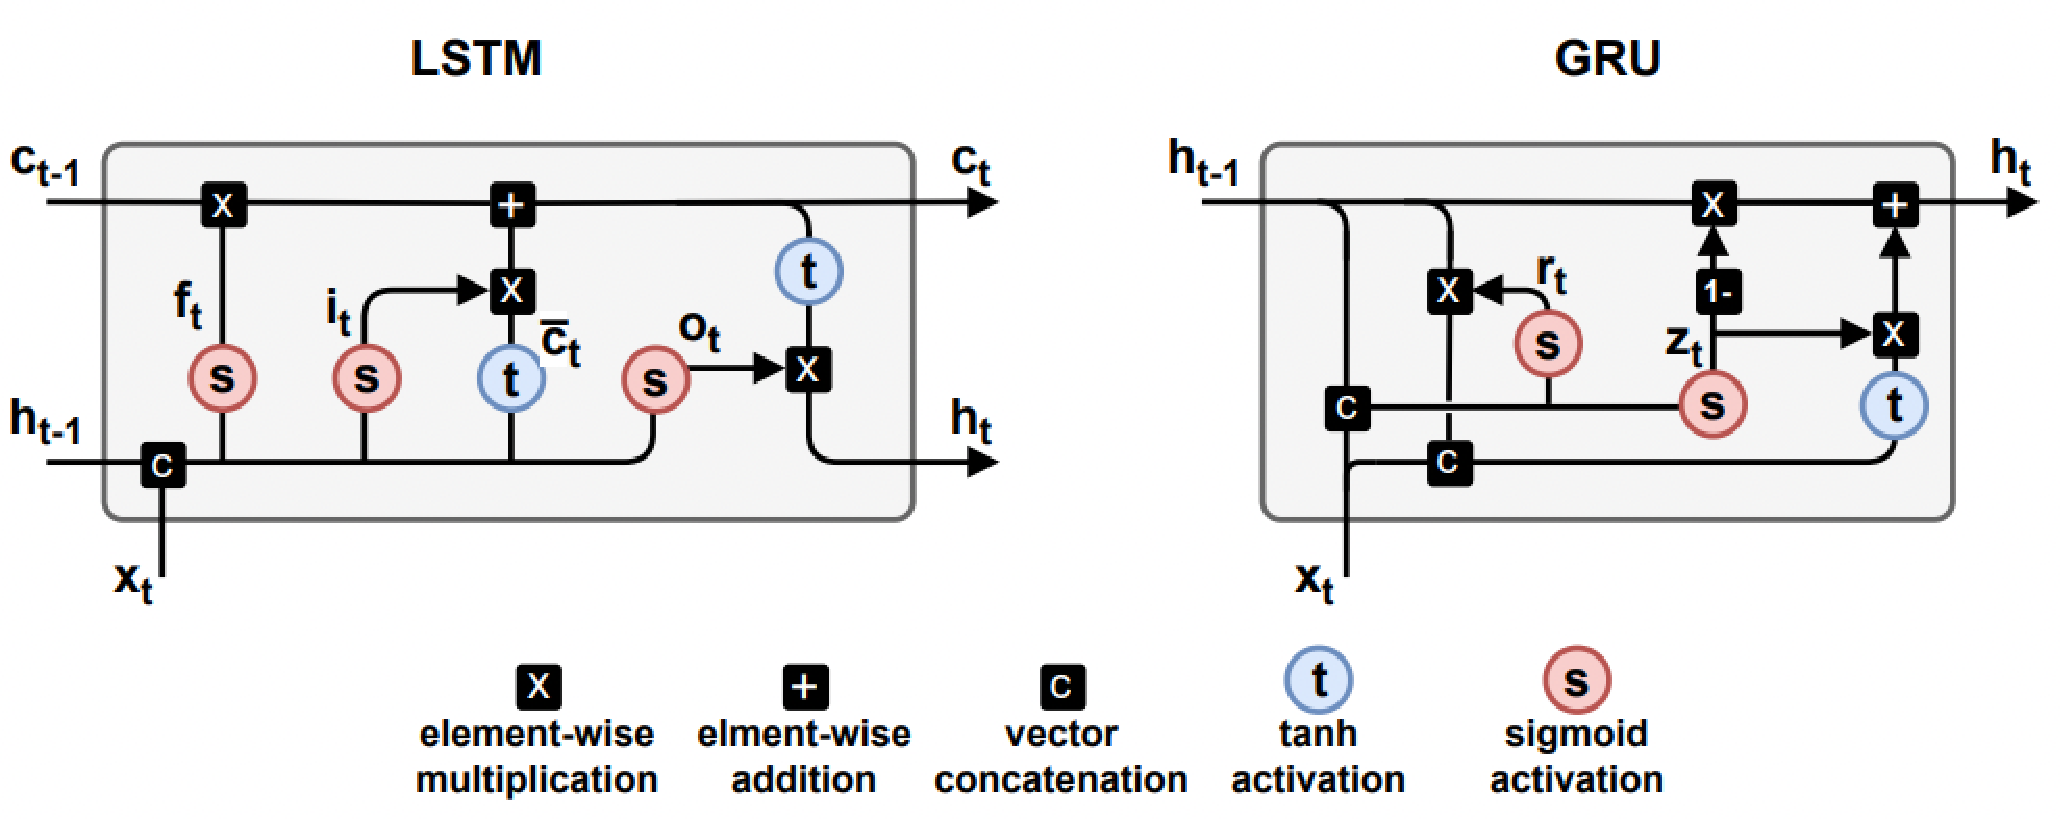
\includegraphics[width=\textwidth]{Figures/sota_5.pdf}

\caption[\textbf{Recurrent Neural Networks (RNNs)}]{\textbf{Recurrent Neural Networks (RNNs):} Schemes representing LSTM and GRU cells. Both show their input $x_t$ and the computation of the new hidden state $h_t$; the LSTM on the left also depicts the additional computation of the cell state $c_t$. (Adapted from \cite{Lafabregue2022End-to-endStudy}).}
\label{fig:2.5}

\end{figure}


\subsubsection{Temporal Convolutional Networks}

Temporal Convolutional Networks (TCNs) are another type of neural network architecture that are designed to handle sequence data, but with a distinctly different approach than RNNs. Instead of maintaining a hidden state over time, TCNs leverage a specialized form of 1-dimensional convolution, which is applied across the temporal dimension of the input data. A key feature of classical TCNs is the use of causal padding to ensure that future data does not influence the current output, thereby preserving the temporal ordering of the sequence. This contrasts with the bidirectional recurrent layers mentioned above, but can be modified in situations in which looking into the future is not necessarily a problem, such as offline time series segmentation. All in all, TCNs are highly versatile and have been used successfully in a variety of applications, such as audio generation and machine translation \cite{Bai2018AnModeling}.

While a simple causal convolution is only able to look back at a history with size linear in the depth of the network, there are several architectural modifications that can be added to solve this issue (Figure~\ref{fig:2.6}). For starters, the use of dilated convolutions enables the model to have an exponentially large receptive field \cite{Oord2016WaveNet:Audio}. Formally, for a 1-D sequence input $X \in R_n$ and a filter $f : \{0, \ldots , k - 1\} \rightarrow R$, the dilated convolution operation $F$ on an element $s$ of the sequence is defined as 

\begin{equation}
F(s) = \sum_{i=0}^{k-1} f(i) \cdot x_{s-d \cdot i}
\label{eq:2.20}
\end{equation}

\noindent where $k$ is the filter size, $d$ is the dilation factor, and $s - d \cdot i$ refers to previous time points. The dilation operation is then equivalent to introducing a fixed step between every two adjacent filters. When $d = 1$, a dilated convolution is equivalent to a regular convolution. Using larger dilations can thus effectively expand the receptive field of the layer. As a corollary, there are two ways to increase the receptive field of the TCN: choosing larger filter sizes k and increasing the dilation factor $d$, where the effective history of one such layer is $(k - 1)d$.

Another popular modification to this architecture is the addition of residual blocks \cite{He2015DeepRecognition}. These consist of branches in the network leading out to a series of transformations $F$, whose outputs are added to the input $x$ of the block: $y = \mathrm{Activation}(x + F(x))$ This effectively allows layers to learn modifications to the identity mapping rather than the entire transformation, which has repeatedly been shown to benefit very deep networks. Within a given residual block, the TCN architecture has two layers of dilated causal convolutions and a non-linearity. Weight normalization and is typically added to the convolutional filters, and dropout is introduced for regularization purposes \cite{Bai2018AnModeling}.

While a powerful framework that is perfectly suitable for the task presented in this thesis, RNNs and TCNs are increasingly being outperformed by models based on self-attention, such as Transformers. In the next section, we will explore what these are and the advantages they offer in terms of receptive field and interpretability, and the disadvantages they may pose when it comes to computing power and data requirements.

\begin{figure}[!thb]
\centering
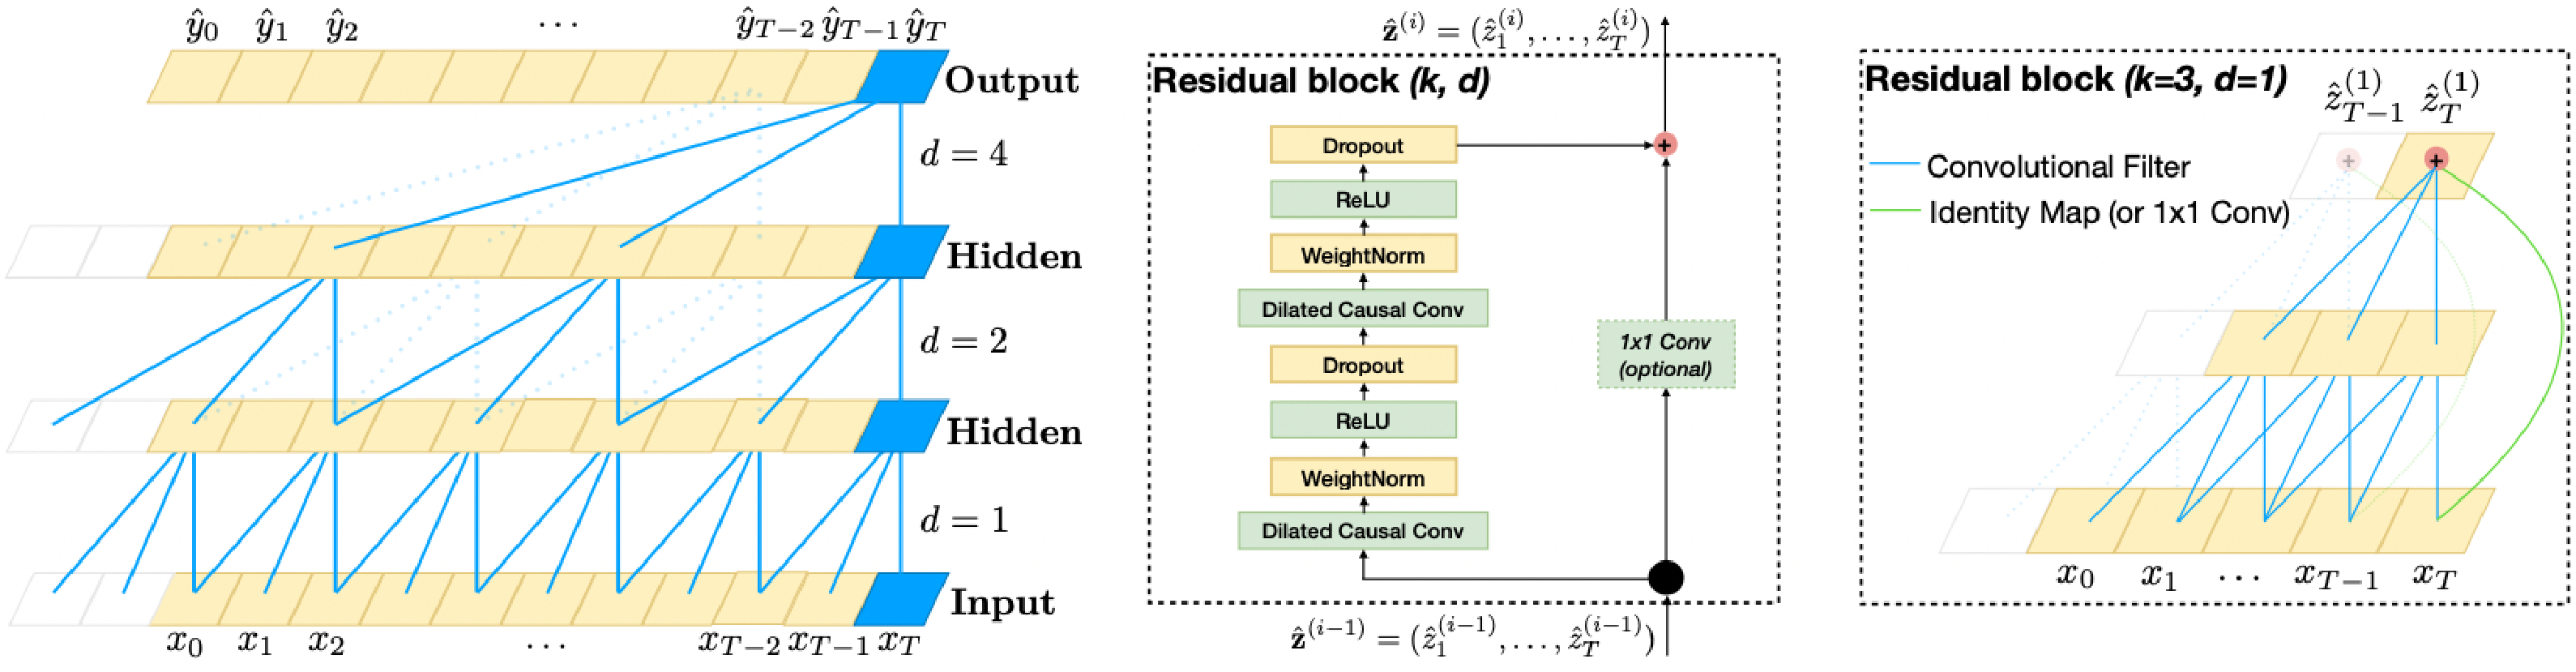
\includegraphics[width=\textwidth]{Figures/sota_6.pdf}

\caption[\textbf{Architectural elements of a Temporal Convolutional Network (TCN)}]{\textbf{Architectural elements of a Temporal Convolutional Network (TCN):} \textbf{Left}: A causal convolution with dilation factors of d = 1, 2, 4, and a filter size of k = 3 is shown. This receptive field can cover all input sequence values. \textbf{Center}: This is a Temporal Convolutional Network (TCN) residual block. When the residual input and output have different dimensions, a 1x1 convolution is introduced. \textbf{Right}: This illustrates a residual connection in a TCN. The blue lines represent filters in the residual function, and the green lines symbolize identity mappings. (Adapted from \cite{Bai2018AnModeling}).}
\label{fig:2.6}

\end{figure}

\subsubsection{Transformer Networks}

The Transformer architecture, introduced by Vaswani et al. in the paper ``Attention is All You Need" \cite{Vaswani2017AttentionNeed} is a novel approach to sequence-to-sequence tasks that significantly improves over traditional Recurrent Neural Networks (RNNs) and (Temporal) Convolutional Neural Networks (TCNs), especially for scenarios where large amounts of data are available.

Transformers are based on the concept of self-attention mechanisms, which allows them to process input sequences in parallel rather than sequentially. This means that sequential information is not directly available to them, and explicit positional encodings are needed to retain order information. The input is thus embedded together with these encodings, and the result is passed through multiple stacked layers of multi-head self-attention and position-wise feed-forward networks. Each layer has residual connections and is followed by layer normalization.

The so called self-attention mechanism works by computing a weighted sum over the input elements and calculating attention scores using a scaled dot-product attention (Figure~\ref{fig:2.7}, left):

\begin{equation}
\text{Attention}(Q, K, V) = \text{softmax}\left(\frac{QK^T}{\sqrt{d_k}}\right)V
\end{equation}

Here, $Q$, $K$, and $V$ are the query, key, and value matrices, respectively, and $d_k$ is the key dimension. This mechanism has several advantages over traditional sequence-aware deep learning methods, since the model can effectively model global dependencies by weighting all time points simultaneously. Moreover, the retrieved attention scores can aid with model interpretability, since they provided a direct measure of features that the model considers important for a particular task.

Furthermore, Transformer networks use a mechanism called Multi-head attention, which applies self-attention multiple times in parallel, concatenating the outputs, and linearly transforming the result (Figure~\ref{fig:2.7}, right):

\begin{align}
\text{MultiHead}(Q, K, V) &= \text{Concat}(\text{head}_1, \dots, \text{head}_h)W^O \\
\text{head}_i &= \text{Attention}(QW_i^Q, KW_i^K, VW_i^V)
\end{align}

\noindent Here, $W^Q$, $W^K$, $W^V$, and $W^O$ are learnable weight matrices.

The Transformer architecture consists of an encoder-decoder structure. The encoder is composed of a stack of identical layers with multi-head self-attention and position-wise feed-forward networks. The decoder has a similar structure but includes an additional multi-head attention mechanism that attends to the encoder's output.

The final output of the Transformer is then produced by a linear layer followed by a $softmax$ layer, yielding a series of probabilities over a set of tokens. 

Transformers have demonstrated exceptional performance in various natural language processing tasks, such as machine translation, text summarization, and question answering. Moreover, they are showing promising results in multi-animal motion tracking models that require complex deidentification of individuals \cite{Lauer2022Multi-animalDeepLabCut}. 

\begin{figure}[!thb]
\centering
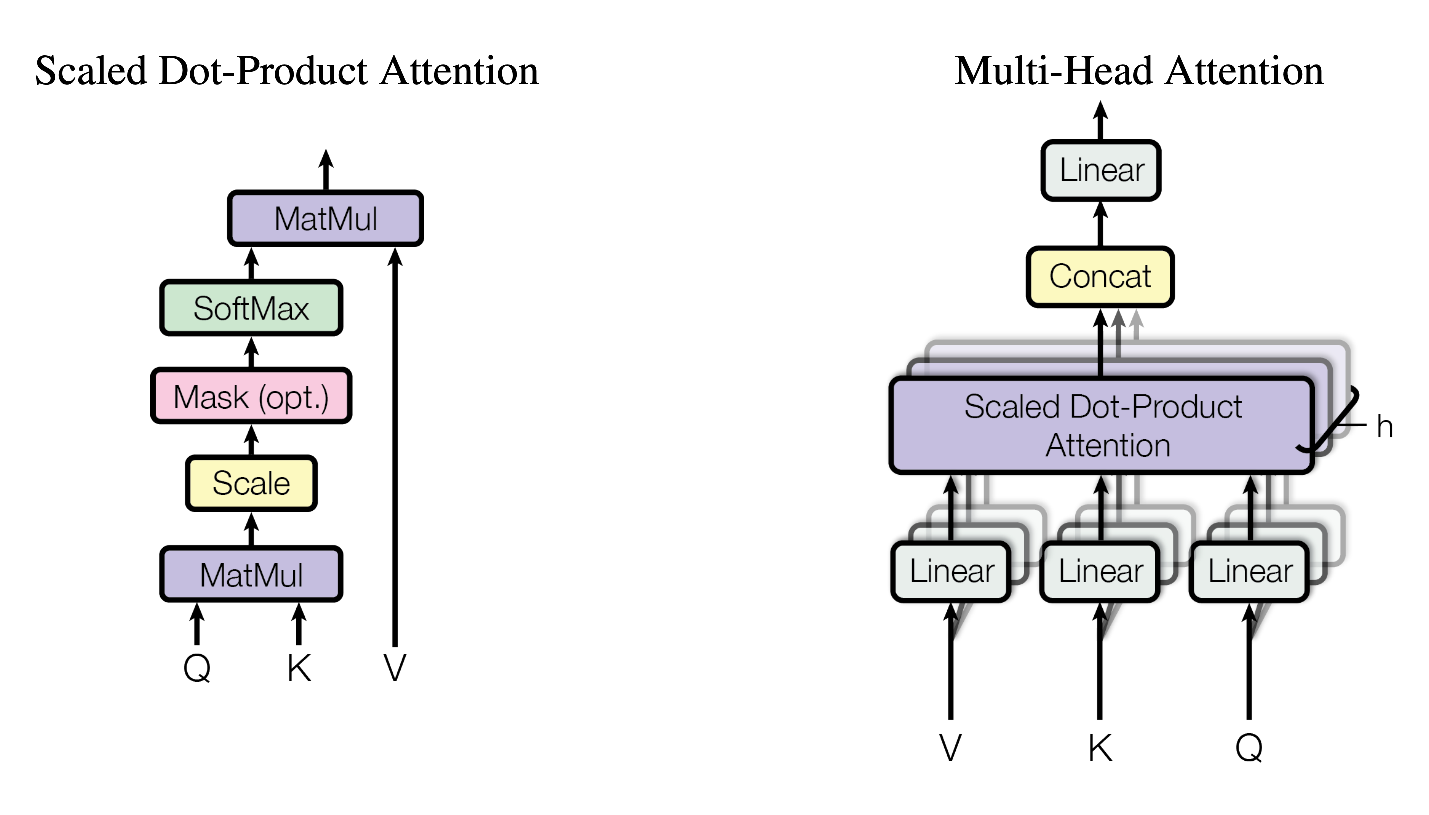
\includegraphics[width=\textwidth]{Figures/sota_7.pdf}

\caption[\textbf{Details on the transformer architecture}]{\textbf{Details on the transformer architecture.} The \textbf{Scaled Dot-Product Attention} operation is depicted on the left, with Queries, Keys, and Values as inputs. The right panel shows the \textbf{Multi-Head Attention} mechanism, which parallelizes several attention heads, in a fashion that can be compared to ensemble learning. (Adapted from \cite{Vaswani2017AttentionNeed}).}
\label{fig:2.7}

\end{figure}

While efficient due to its highly parallelizable architecture, Transformers are well known for requiring vast amounts of data and computing power to work in practice. While the current thesis includes experiments using models akin to these, data sizes achieved in behavioral experiment setups are arguably too small for the task.
Now that several time series processing architectures and clustering methods have been presented, the next sections will delve into deployed algorithms for motion time series segmentation that use some of the discussed approached.

\section{Segmenting behavior: exploring available approaches}

Since the advent of DeepLabCut and SLEAP, a significant number of tools designed to leverage marker-less pose estimation have been introduced. The subsequent sections explore three such tools, all of which provide approaches to behavioral segmentation. These are B-SOiD \cite{Hsu2021B-SOiDBehaviors}, which utilizes traditional clustering techniques on features extracted over time, MoSeq \cite{Weinreb2023Keypoint-MoSeq:Dynamics} which relies on Hidden Markov Models, and VAME, which takes advantage of post-hoc clustering on embeddings generated through deep neural networks.

\subsubsection{B-SOiD: time series clustering using guided representations}

B-SOiD was presented in 2021 by Alexander Hsu and Eric Yttri \cite{Hsu2021B-SOiDBehaviors}. It works by extracting a series of descriptive kinematic features from the motion tracking time series obtained with DeepLabCut or SLEAP, including displacement, angular change, and distances between body parts. These features are then aggregated over a sliding window of 60\,ms (30\,ms before and 30\,ms after the frame of interest). Furthermore, the original data is downsampled to 10 frames per second (FPS), which the authors claim helps increase the signal-to-noise when it comes to distinguishing real movement from label jittering.

Once these features are extracted, their dimensionality is reduced using PCA, with a number of components such that they explain 70\,\% of the variance in the motion tracking data. UMAP is then applied with the same number of components to get a representation that enforces local aggregation, and motion clusters are obtained using HDBSCAN. This algorithm is a particularly good approach when it comes to detecting outliers, since it can remove subthreshold densities \cite{McInnes2017Hdbscan:Clustering}. Moreover, it does not require the user to select the number of clusters ad-hoc.

Once the clusters are obtained, B-SOiD trains a multi-class random forest from the original statistics to the cluster labels assigned by HDBSCAN, which is shown to improve generalizability to unseen data. The trained models can then quickly assign data points to clusters and enable further analysis (Figure~\ref{fig:2.8}).

While a simple approach, B-SOiD is shown to work quite well in many popular scenarios including not only rodents, but also flies and humans, to name a few. Moreover, it does not require expensive hardware to train in small or medium datasets, and further developments use the obtained clusters as the starting point to train even more generalizable classifiers in an active learning framework \cite{Schweihoff2022A-SOiDBehavior}. The simplicity of the pipeline has its limitations, however, as the extracted features are assumed to capture most variation in the detected animal's dynamics. In rodents, this means that direct access to paw movement is needed to achieve good results, which is only achieved with bottom-up videos (where the animals are filmed from below through a glass floor). This is non-standard practice in many labs, since it requires special hardware and it was shown to stress the animals \cite{Miranda2023IncreasingBehaviors}. Furthermore, no explicit information about dynamics is used, which can hurdle the flexibility of the retrieved clusters, and only single animals are supported.

\begin{figure}[!thb]
\centering
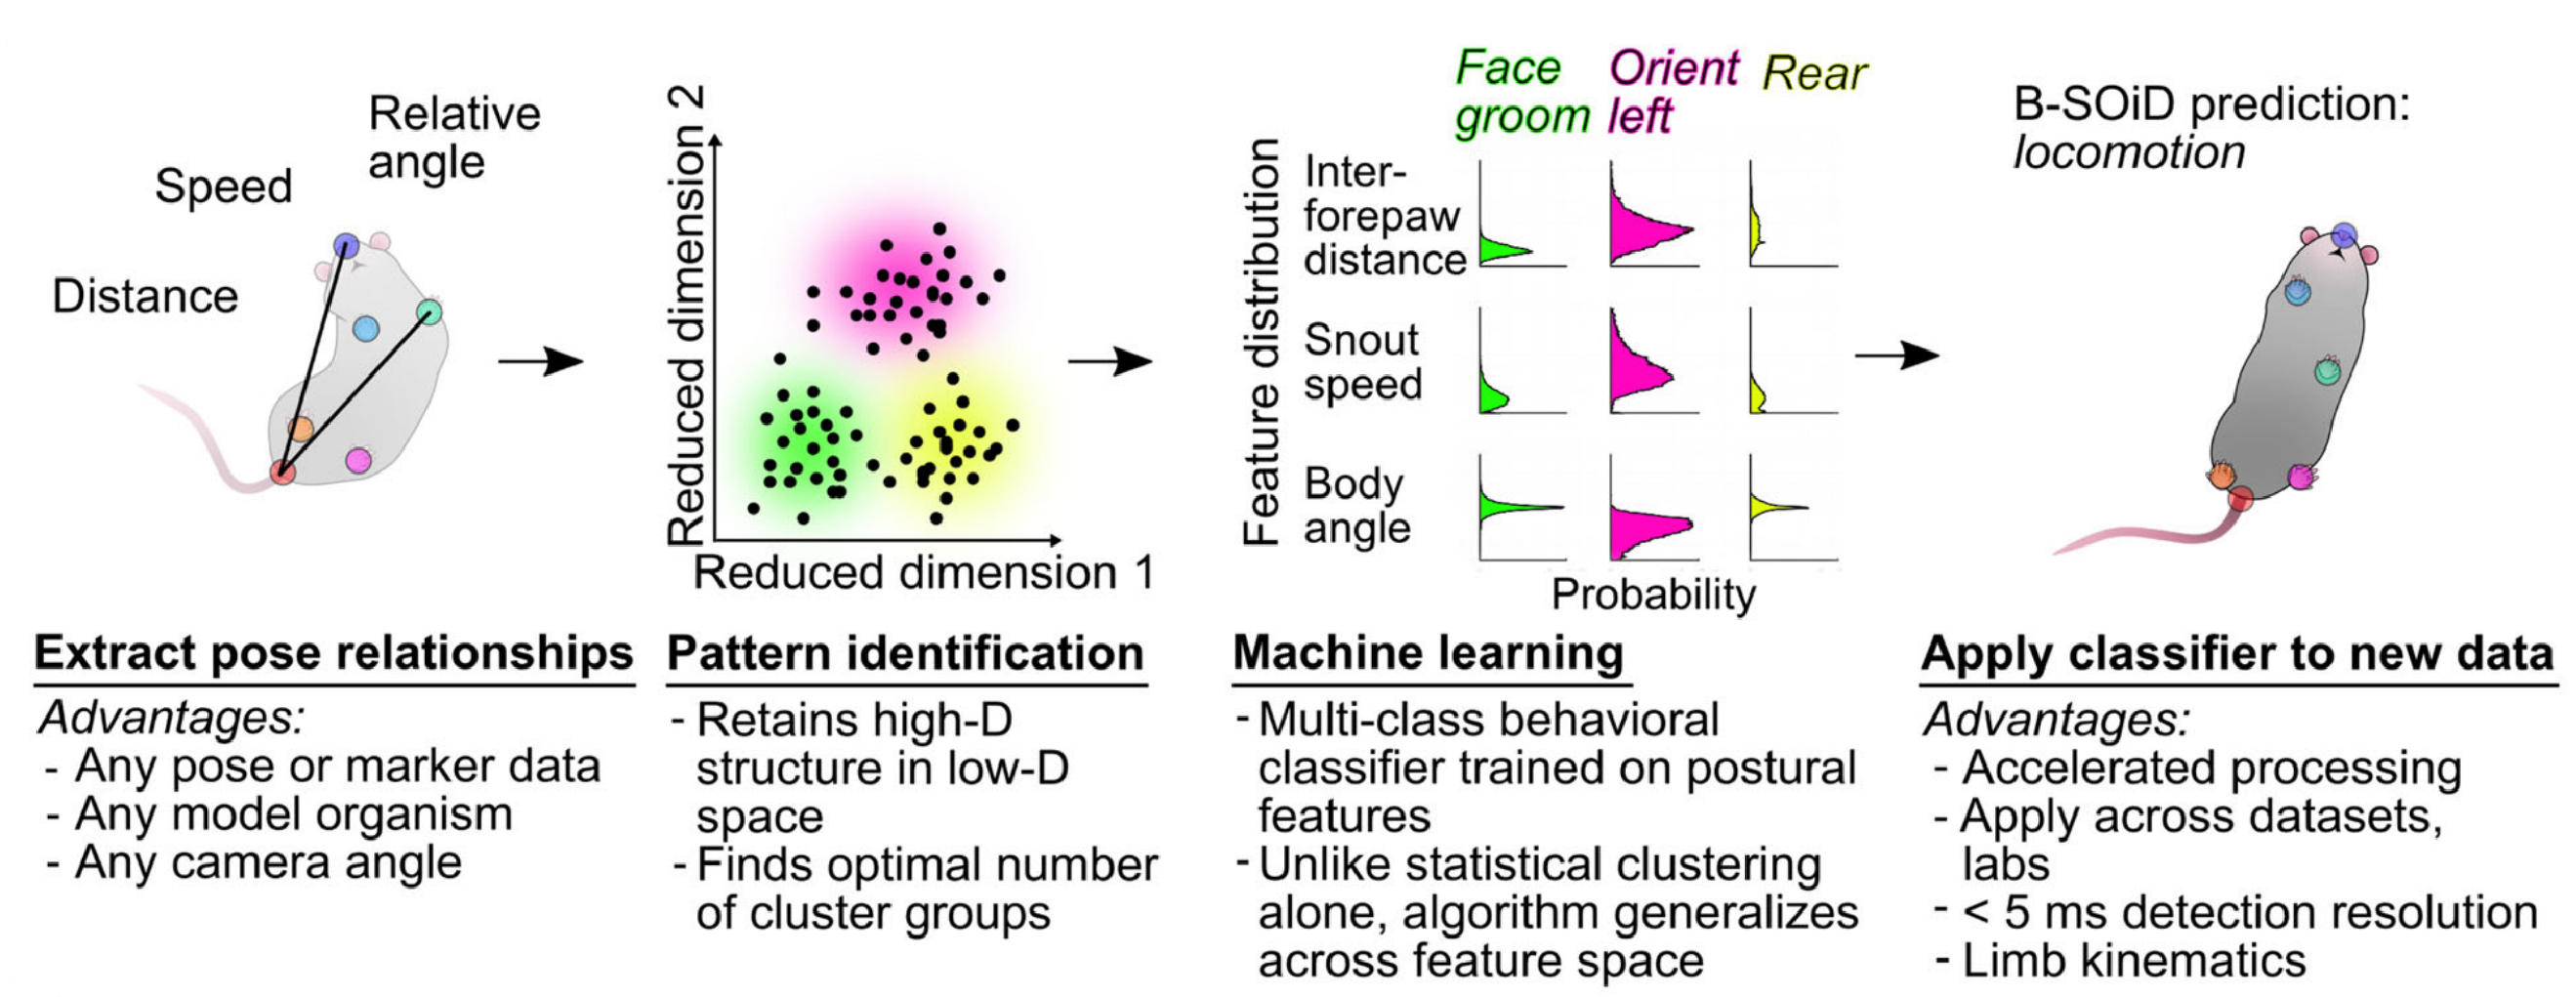
\includegraphics[width=\textwidth]{Figures/sota_8.pdf}

\caption[\textbf{Overview of the B-SOiD pipeline}]{\textbf{Overview of the B-SOiD pipeline.} Once the pose relationships that characterize behaviors are extracted, B-SOiD applies a non-linear transformation (UMAP) to preserve high-dimensional postural time-series data in a lower-dimensional space, and HDBSCAN is subsequently used for cluster identification. The spatiotemporal features that have been clustered serve as inputs for training a random forest classifier, which can then be employed to promptly predict behavioral categories in any comparable data set. Once trained, the model will segment any dataset into the same classes. (Adapted from \cite{Hsu2021B-SOiDBehaviors}).}
\label{fig:2.8}

\end{figure}

\subsubsection{MoSeq: motion clustering with Autoregressive Hidden Markov Models}

MoSeq (motion sequencing) is a Hidden Markov Model approach for behavioral segmentation introduced by Sandeep Robert Datta and collaborators back in 2019 \cite{Datta2015QA:Behavior}. To solve the short range dependencies introduced by the Markov assumption, the authors use an Autoregressive Hidden Markov Model (AR-HMM) approach, which relies on an HMM where the observation model (the model that generates the outputs from the hidden states) is an autoregressive model in itself. In other words, the models are designed so that each hidden state has an autoregressive (AR) model associated with it, which means that the current output not only depends on the current hidden state, but also on previous outputs.

While the authors originally demonstrated high capabilities of this approach for depth sensing camera setups, the original algorithms were not capable of dealing with keypoint estimation data coming from regular video. In a recent preprint \cite{Weinreb2023Keypoint-MoSeq:Dynamics}, the group behind MoSeq introduced a variant which decouples keypoint motion to actual animal motion and label jitter, which the authors identify as the main culprit of previous versions' poor performance in these settings (Figure \ref{fig:2.9}). 

\begin{figure}[!thb]
\centering
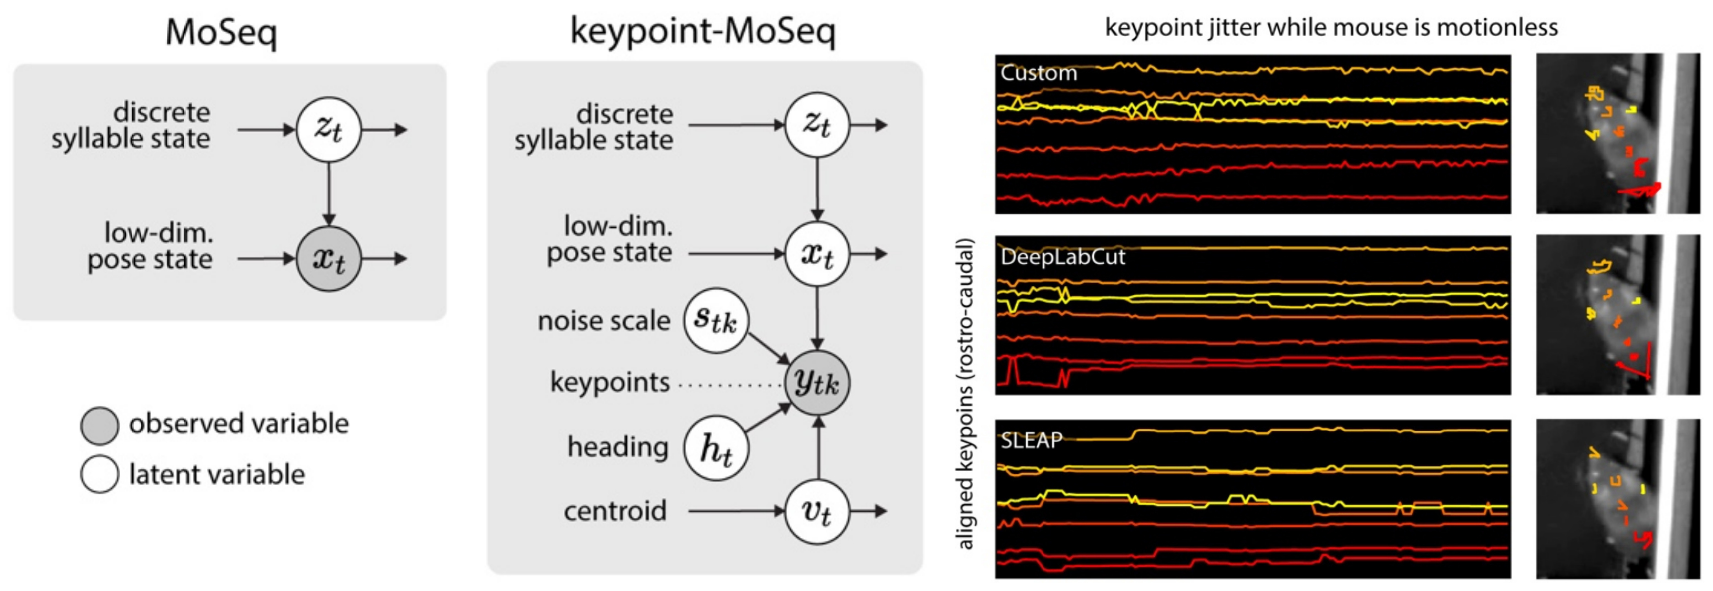
\includegraphics[width=\textwidth]{Figures/sota_9.pdf}

\caption[\textbf{MoSeq: motion clustering with Autorregressive Hidden Markov Models}]{\textbf{MoSeq: motion clustering with Autorregressive Hidden Markov Models.} \textbf{a}: Graphical models showcasing both MoSeq and a new hierarchical model known as “keypoint-MoSeq” are presented. In both models, a discrete syllable sequence dictates the dynamics of a low-dimensional pose state. The pose state is either determined using PCA (as demonstrated in “MoSeq”, left) or inferred from keypoint observations in relation to the animal’s centroid and heading, as well as a noise scale to account for keypoint detection errors (as demonstrated in “keypoint-MoSeq”, right). \textbf{b}: This is an example of keypoint jitter from three distinct keypoint tracking methods during a 5-second interval when the mouse was stationary. The left side shows keypoint trajectories aligned egocentrically, whereas the right side shows the path traced by each keypoint during the interval. (Adapted from \cite{Weinreb2023Keypoint-MoSeq:Dynamics}).}
\label{fig:2.9}

\end{figure}

\subsubsection{VAME: Variational Animal Motion Embeddings}

Finally, Kevin Luxem and colleagues introduced VAME (Variational Animal Motion Embeddings) in 2022 (Figure \ref{fig:2.10}). The package, implemented in Python and PyTorch, relies on deep neural networks to embed motion tracking time series. In their pipeline, a variational autoencoder maps the input to an unimodal multivariate Gaussian latent space, and post-hoc clustering is applied to the embeddings using a Hidden Markov Model. Moreover, the architecture has two decoders: one trained to minimize the reconstruction error with the input (reconstruction decoder), and one that aims to predict the next unseen timepoint (prediction decoder), which helps to regularize the obtained embeddings. In their paper \cite{Luxem2022IdentifyingMotion}, the authors show how their models can robustly detect shifts in behavior in rodents with beta amyloidosis. While results are promising, the authors only demonstrate the capabilities of the software using bottom-up videos with access to the paws' positions at all times.

\begin{figure}[H]
\centering
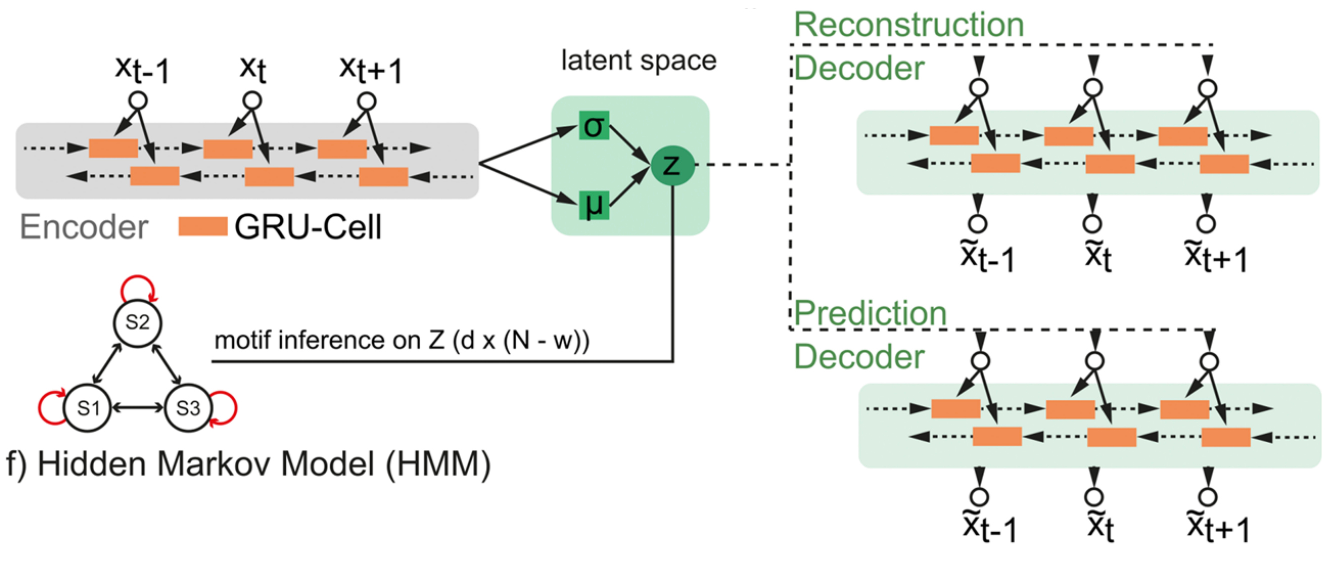
\includegraphics[width=\textwidth]{Figures/sota_10.pdf}

\caption[\textbf{VAME: Variational Animal Motion Embeddings}]{\textbf{VAME: Variational Animal Motion Embeddings.} Frames are aligned egocentrically, and trajectory samples are fed to a
recurrent variational autoencoder model. The fully trained model functions like a dynamical system, from which motifs are deduced using a Hidden-Markov-Model. (Adapted from \cite{Luxem2022IdentifyingMotion}).}
\label{fig:2.10}

\end{figure}

\clearpage

\section{Main contributions of this thesis to the field}

All in all, this thesis aims to build on the presented state of the art in three main ways.

\subsection{Implementation and testing of novel deep clustering algorithms for unsupervised behavioral segmentation}

As a first goal, this thesis aims to present new variants of deep clustering algorithms (that is, models that couple deep neural network embeddings and clustering) for multivariate time series data, specifically tailored to work with rodent motion tracking. %A comparison between the state of the art and the proposed algorithms will be presented in chapter \ref{chap:discussion}.

\subsection{Deployment of the developed algorithms to the community}

Aside from implementing and testing these developed algorithms, an important goal of this work is to deploy them in a packaged manner for the community to use with their own data. Along these lines the DeepOF (Deep Open Field) package was born, a Python suite with tools for processing, annotation, and deep clustering of rodent motion tracking data. Chapter \ref{chap:joss} will delve into the design philosophy of DeepOF, its inner workings, and include a paper published in the \href{https://joss.theoj.org/}{Journal of Open Source Software} (JOSS), which included detailed code, documentation, and testing pipeline reviews.

\subsection{Application of the developed algorithms to the characterization of Chronic Social Defeat Stress}

As introduced earlier in chapter \ref{chap:introduction}, all developed algorithms were applied to the characterization of Chronic Social Defeat Stress as a case study. Chapter \ref{chap:natcomm} will delve into this, presenting the deployed algorithms in detail, and showcasing the application of DeepOF to the supervised and unsupervised characterization of the provided animal model, as a paper published in \href{https://www.nature.com/ncomms/}{Nature Communications}.